\documentclass[11pt, letterpaper]{article}

% --- PAQUETES ---
\usepackage[utf8]{inputenc}
\usepackage[T1]{fontenc}
\usepackage[spanish, es-noshorthands]{babel}
\usepackage[top=2cm, bottom=2.2cm, left=2.2cm, right=2.2cm]{geometry}
\usepackage{graphicx}
\usepackage{amsmath}
\usepackage{amssymb}
\usepackage{enumitem}
\usepackage{xcolor} 
\usepackage{fancyhdr}
\usepackage{eso-pic}

% --- FUENTE SISTEMA ---
\usepackage{helvet}
\renewcommand{\familydefault}{\sfdefault}

% =================================================================
% CONFIGURACIÓN PARA MOSTRAR / OCULTAR RESPUESTAS
% =================================================================
\newif\ifmostrarrespuestas

% ---> MODO PROFESOR (Muestra respuestas en azul): Deja la siguiente línea sin comentar.
\mostrarrespuestastrue 

% ---> MODO ESTUDIANTE (Oculta respuestas y no deja espacio): Comenta la línea anterior añadiendo un % al inicio.
%\mostrarrespuestasfalse

% --- COMANDO DE RESPUESTAS ---
\newcommand{\respuesta}[1]{
	\ifmostrarrespuestas
	\par\vspace{0.2cm}
	\textbf{\textcolor{blue}{Solución:}} \textcolor{blue}{#1}
	\vspace{0.4cm}
	\else
	% No imprime nada en modo estudiante para mantener la guía limpia
	\fi
}
% =================================================================

% Fondo institucional (opcional, ajusta la ruta si es necesario)
% \AddToShipoutPictureBG{
	% 	\AtPageLowerLeft{
		% 		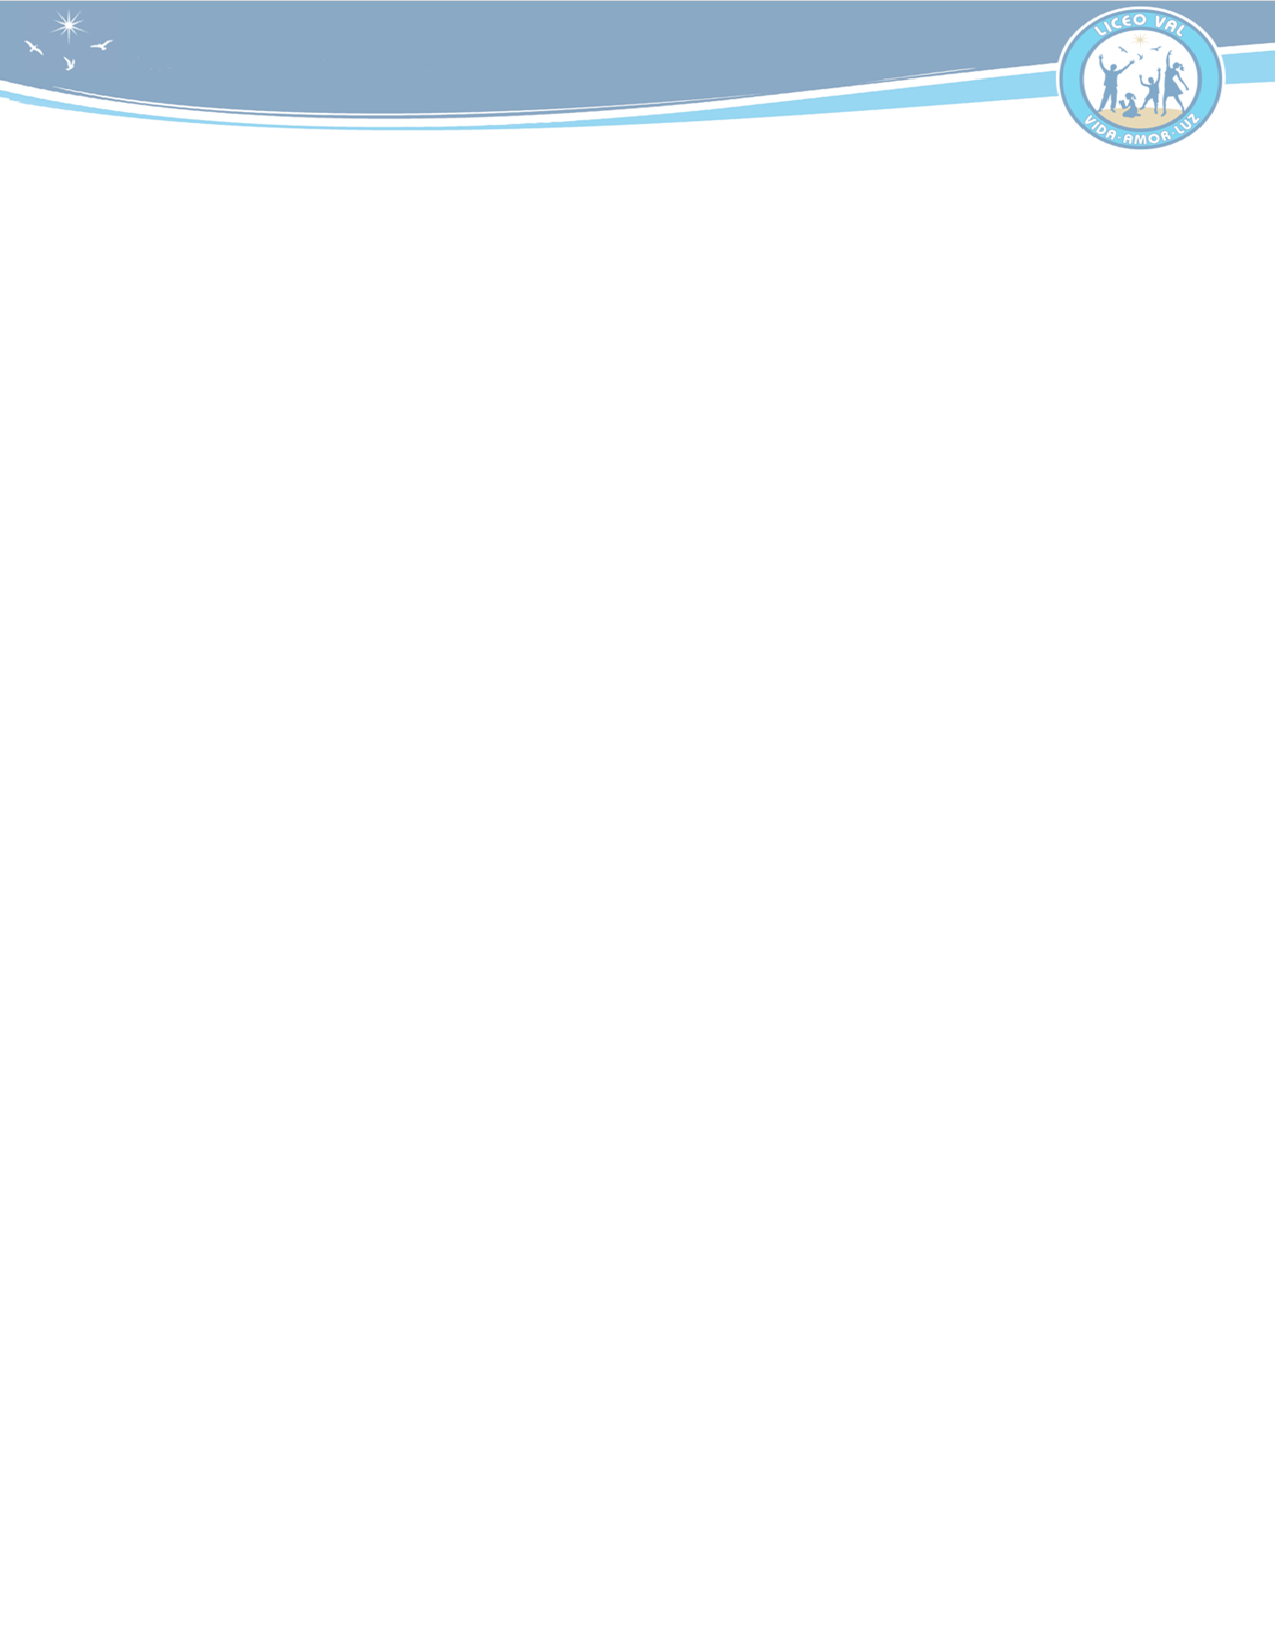
\includegraphics[width=\paperwidth,height=\paperheight,keepaspectratio=false]{../../FondoVAL.pdf}
		% 	}
	% }

% --- CONFIGURACIÓN DE PÁGINA ---
\pagestyle{fancy}
\fancyhf{}
\fancyhead[L]{\footnotesize \color{gray} LICEO V.A.L. -- DEPARTAMENTO DE CIENCIAS BÁSICAS}
\fancyhead[R]{\footnotesize \color{gray} FÍSICA 11º}
\fancyfoot[C]{\footnotesize \color{gray} Página \thepage}
\renewcommand{\headrulewidth}{0.4pt}
\renewcommand{\footrulewidth}{0pt}

\begin{document}
	
	% --- ENCABEZADO ---
	\begin{center}
		{\Large \textbf{LICEO V.A.L. (Vida, Amor, Luz)}}\\[0.1cm]
		{\large \textbf{DEPARTAMENTO DE CIENCIAS BÁSICAS}}\\[0.1cm]
		{\large \textbf{TALLER DE REFUERZO: FÍSICA 11º (RUTA REGULAR)}}\\[0.1cm]
		\hfill \textbf{Código: 11 F -- 03. E} 
		\ifmostrarrespuestas \textcolor{blue}{\textbf{(VERSIÓN PROFESOR)}} \else \textbf{(VERSIÓN ESTUDIANTE)} \fi
	\end{center}
	
	\vspace{0.3cm}
	\noindent \textbf{Nombre:} \underline{\hspace{8.5cm}} \textbf{Fecha:} \underline{\hspace{3cm}}
	
	%\vspace{0.4cm}
	%\noindent \textit{Este taller exige un alto nivel de abstracción matemática y análisis deductivo para modelar fenómenos ondulatorios, en concordancia con el compromiso de excelencia académica establecido en el Manual de Convivencia Liceo VAL 2026. Todas las respuestas deben estar rigurosamente justificadas.}
	\vspace{0.6cm}
	
	% --- PREGUNTAS ---
	\begin{enumerate}[leftmargin=*, itemsep=0.8cm]
		
		\item  Una onda mecánica transversal viaja por un medio elástico ideal y se modela mediante la función $y(x,t) = 4.5 \sin(4x + 6\pi t)$ en unidades del SI. Determine mediante análisis deductivo:
		\begin{enumerate}[label=\alph*., itemsep=0.2cm]
			\item El periodo ($T$) y la amplitud ($A$).
			\item La velocidad de propagación de la onda ($v$).
		\end{enumerate}
		\respuesta{
			a) De la estructura $y(x,t) = A \sin(kx + \omega t)$, extraemos: $A = 4.5 \text{ m}$. La frecuencia angular es $\omega = 6\pi \text{ rad/s}$. Sabiendo que $T = \frac{2\pi}{\omega}$, tenemos $T = \frac{2\pi}{6\pi} = \frac{1}{3} \text{ s} \approx 0.33 \text{ s}$.\\
			b) El número de onda es $k = 4 \text{ rad/m}$. La velocidad de propagación es $v = \frac{\omega}{k} = \frac{6\pi}{4} = \frac{3\pi}{2} \text{ m/s} \approx 4.71 \text{ m/s}$.
		}
		
		\item  Una fuente genera $20 \text{ pulsos}$ en $5 \text{ segundos}$, produciendo ondas de $15 \text{ cm}$ de longitud con una amplitud de $0.1 \text{ m}$.
		\begin{enumerate}[label=\alph*., itemsep=0.2cm]
			\item Calcule la frecuencia angular ($\omega$) y el número de onda ($k$).
			\item Escriba la ecuación formal de la onda $y(x,t)$ asumiendo que se desplaza hacia la derecha.
		\end{enumerate}
		\respuesta{
			a) Frecuencia $f = \frac{20}{5} = 4 \text{ Hz}$. La frecuencia angular $\omega = 2\pi f = 8\pi \text{ rad/s}$. La longitud de onda es $\lambda = 0.15 \text{ m}$, por lo que el número de onda $k = \frac{2\pi}{\lambda} = \frac{2\pi}{0.15} = \frac{40\pi}{3} \text{ rad/m} \approx 41.89 \text{ rad/m}$.\\
			b) Como se desplaza hacia la derecha, el signo interno es negativo: $y(x,t) = 0.1 \sin\left(\frac{40\pi}{3} x - 8\pi t\right)$.
		}
		
		\item  La onda descrita en el punto 2 incide sobre un nuevo medio material donde su velocidad disminuye a $0.4 \text{ m/s}$. Demuestre matemáticamente qué sucede con la frecuencia de la onda refractada y justifique físicamente por qué esta magnitud es un invariante del sistema.
		\respuesta{
			Físicamente, la frecuencia está determinada exclusivamente por la fuente generadora de la vibración inicial, no por el medio material. Por tanto, la frecuencia en el medio 2 será exactamente igual a la del medio 1: $f_2 = f_1 = 4 \text{ Hz}$. La magnitud es invariante debido a la conservación del número de frentes de onda que cruzan la interfaz por unidad de tiempo.
		}
		
		\item Utilizando los datos y la frecuencia demostrada en el punto 3, determine la nueva longitud de onda ($\lambda_2$) en el medio refractado. Demuestre la relación de proporcionalidad directa entre la velocidad y la longitud de onda.
		\respuesta{
			Sabiendo que $v_2 = 0.4 \text{ m/s}$ y que la frecuencia se mantiene constante en $f = 4 \text{ Hz}$: \\
			$\lambda_2 = \frac{v_2}{f} = \frac{0.4 \text{ m/s}}{4 \text{ Hz}} = 0.1 \text{ m}$. \\
			Si $v = \lambda \cdot f$ y $f$ es constante, $v$ y $\lambda$ son directamente proporcionales. Al disminuir la velocidad en el nuevo medio, la longitud de onda debe disminuir proporcionalmente.
		}
		
		\item Un rayo de luz incide desde el aire con un ángulo de incidencia de $40^\circ$ a un medio con un índice de refracción de $1.8$. Determine:
		\begin{enumerate}[label=\alph*., itemsep=0.2cm]
			\item El ángulo de refracción.
			\item La velocidad de propagación de la onda electromagnética en este medio.
		\end{enumerate}
		\respuesta{
			a) Ley de Snell: $n_1 \sin(\theta_1) = n_2 \sin(\theta_2) \implies 1 \cdot \sin(40^\circ) = 1.8 \cdot \sin(\theta_2)$.\\
			$\sin(\theta_2) = \frac{0.6428}{1.8} \approx 0.357 \implies \theta_2 = \arcsin(0.357) \approx 20.92^\circ$.\\
			b) Índice $n = \frac{c}{v} \implies v = \frac{c}{n} = \frac{3 \times 10^8 \text{ m/s}}{1.8} \approx 1.67 \times 10^8 \text{ m/s}$.
		}
		
		\item Para el mismo sistema del punto 5, si el rayo viajara en sentido inverso (del medio de índice $1.8$ hacia el aire), ¿cuál sería el ángulo límite o crítico para que se presente reflexión interna total?
		\respuesta{
			El ángulo límite ($\theta_c$) ocurre cuando el ángulo de refracción es $90^\circ$ ($\sin 90^\circ = 1$).\\
			$n_1 \sin(\theta_c) = n_2 \sin(90^\circ) \implies 1.8 \sin(\theta_c) = 1(1) \implies \sin(\theta_c) = \frac{1}{1.8} \approx 0.555$.\\
			$\theta_c = \arcsin(0.555) \approx 33.75^\circ$.
		}
		
		\item Una onda armónica definida por la ecuación $y(x,t) = 0.5 \sin(2\pi x - 10\pi t)$ (en el SI) viaja por un Medio 1 e incide sobre un Medio 2 con un ángulo de $45^\circ$. Si el ángulo de refracción medido en el Medio 2 es de $30^\circ$, determine la velocidad de la onda en el Medio 2.
		\respuesta{
			Primero extraemos la velocidad del Medio 1: $\omega = 10\pi$, $k = 2\pi \implies v_1 = \frac{\omega}{k} = \frac{10\pi}{2\pi} = 5 \text{ m/s}$.\\
			Usamos la Ley de Snell en términos de velocidades: $\frac{\sin(\theta_1)}{v_1} = \frac{\sin(\theta_2)}{v_2}$.\\
			$\frac{\sin(45^\circ)}{5} = \frac{\sin(30^\circ)}{v_2} \implies \frac{0.707}{5} = \frac{0.5}{v_2} \implies v_2 = \frac{5 \cdot 0.5}{0.707} \approx 3.53 \text{ m/s}$.
		}
		
		\item Un rayo de luz incide desde el aire con un ángulo de incidencia de $38^\circ$ a un medio líquido en el que se refracta con un ángulo de refracción de $28^\circ$.
		\begin{enumerate}[label=\alph*., itemsep=0.2cm]
			\item Calcule el índice de refracción absoluto del líquido.
			\item Determine la velocidad de la luz en dicho líquido.
		\end{enumerate}
		\respuesta{
			a) $n_1 \sin(\theta_1) = n_2 \sin(\theta_2) \implies 1 \cdot \sin(38^\circ) = n_2 \cdot \sin(28^\circ)$.\\
			$n_2 = \frac{\sin(38^\circ)}{\sin(28^\circ)} = \frac{0.615}{0.469} \approx 1.31$.\\
			b) $v = \frac{c}{n} = \frac{3 \times 10^8 \text{ m/s}}{1.31} \approx 2.29 \times 10^8 \text{ m/s}$.
		}
		
		\item Si una onda electromagnética ingresa a un cristal provocando que su longitud de onda se reduzca a la tercera parte de su valor original en el vacío, ¿cuál es el índice de refracción del cristal? Justifique algebraicamente partiendo de la ecuación $v = \lambda \cdot f$.
		\respuesta{
			En el vacío, la velocidad es $c = \lambda_0 \cdot f$. En el cristal, la frecuencia se mantiene ($f$), por lo que la nueva velocidad es $v = \lambda_2 \cdot f$.\\
			Como $\lambda_2 = \frac{\lambda_0}{3}$, tenemos que $v = \left(\frac{\lambda_0}{3}\right) f = \frac{\lambda_0 \cdot f}{3} = \frac{c}{3}$.\\
			El índice de refracción es la razón de velocidades: $n = \frac{c}{v} = \frac{c}{\frac{c}{3}} = 3$. El índice es 3.
		}
		
		\item Responda falso (\textbf{F}) o verdadero (\textbf{V}) y justifique su respuesta con rigor físico-matemático:
		\begin{enumerate}[label=\alph*., itemsep=0.2cm]
			\item No existen medios materiales en los que la luz presente valores de velocidad mayores a $3 \times 10^8 \text{ m/s}$. \underline{\hspace{1cm}}
			\item Al refractarse una onda sonora y pasar del aire al agua, el cambio en su dirección se debe exclusivamente a que su frecuencia se altera en el nuevo medio. \underline{\hspace{1cm}}
		\end{enumerate}
		\respuesta{
			a) \textbf{V}. De acuerdo con la teoría de la relatividad, la velocidad máxima en el universo es $c$ ($3 \times 10^8 \text{ m/s}$) y ocurre en el vacío. Cualquier medio material tiene un $n > 1$, lo que matemáticamente obliga a que $v = c/n$ sea siempre menor a $c$.\\
			b) \textbf{F}. La desviación (cambio de dirección) ocurre por el cambio en la \textbf{velocidad} de propagación y por ende de su longitud de onda. La frecuencia es invariante y no se altera al cambiar de medio.
		}
		
	\end{enumerate}
	
\end{document}